\cleardoublepage

\section{理论基础}
这部分,我们首先将介绍图及其代数性质,然后介绍图信号的定义,最后介绍用于图卷积神经网络
设计的频谱理论和空间理论。对于大部分的图卷积神经网络的任务,我们默认初始的图信号和图结构
是已知的,图卷积层是待设计的,图卷积层的设计依赖已知的图结构。输入的图信号经过图卷积层得
到一个新的图信号,整个过程反复几次,如图\ref{2-1}所示,最终获得一个期望的输出。
\begin{figure}[ht]
    \centering
    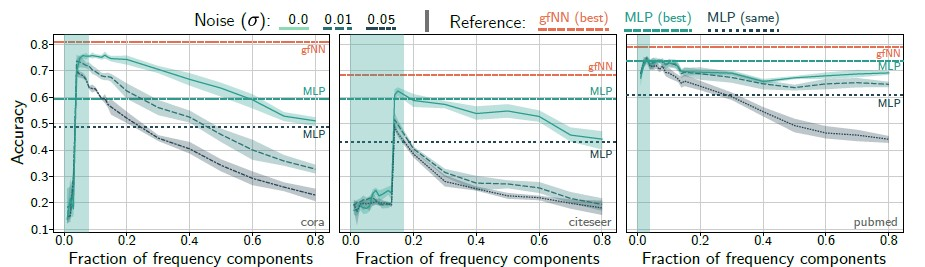
\includegraphics[width=12cm]{theory/1.jpg}
    \caption{\label{2-1}图信号经过图卷积层}
\end{figure}

\subsection{图及其代数性质}
在数学的图论分支中,图可以用来表示事物之间的关系。一张图$\ G = (V , E) $由节点$\ V = \left \{ v_{0},\cdots,v_{N-1} \right \} $
和连接这些节点的边$\ E = \left \{ e_{0}, \cdots ,e_{M-1} \right \} $组成。如图\ref{2-2},图结构就可以表示为节点集
$\ V = \left \{ v_{0}, v_{1},v_{2},v_{3},v_{4} \right \} $和边集$\ E = \left \{ \langle v_0,v_1,5 \rangle , \cdots, \langle v_5,v_2,1 \rangle \right \} $。
通过判断边是否有方向,我们可以将图分为有向图和无向图,在有向图中,一个节点相关联的边可以分为出边和入边,一条边相关联的两个点可以分为
起点和终点。此外,我们还将一个节点所相关联的总边数定义为节点的度,一个节点以该点为起点的边数称为出度,以该点为终点的边数称为入度。
\begin{figure}[ht]
    \centering
    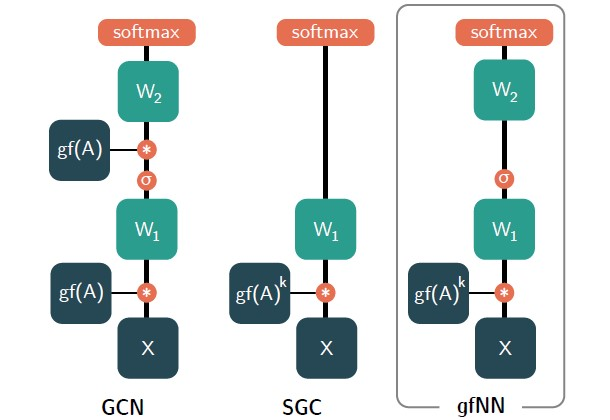
\includegraphics[width=6cm]{theory/2.jpg}
    \caption{\label{2-2}图结构}
\end{figure}

对于节点和节点之间的连通关系,如果这两节点可以通过$K$条边相连,我们称它们之间$K$阶相连,或称它们的关系为K-hop。
如图\ref{2-3},我们默认每个节点都自连,黑颜色的表示当前节点,红颜色的表示与它K阶相连的节点。
\begin{figure}[ht]
    \centering
    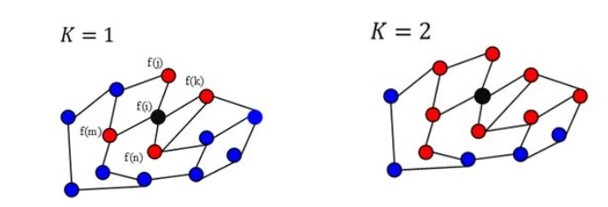
\includegraphics[width=12cm]{theory/3.jpg}
    \caption{\label{2-3}K-hop连通图}
\end{figure}

每个有限图都对应于一个邻接矩阵$A \in R^{N \times N}$,$N$是图上节点的数量,它用矩阵元素是否为零表示各点之间是否有连边。
\begin{equation*}
    A_{m,n} = \begin{cases}1,if\left \langle v_{n}, v_{m} \right \rangle  \in E
     \\0,otherwise
    \end{cases}
\end{equation*}
无向图的邻接矩阵是对称矩阵,如图\ref{2-4};有向图的邻接矩阵可以是不对称的,如图\ref{2-5}。
% \begin{figure}[htbp]
%     \centering
%     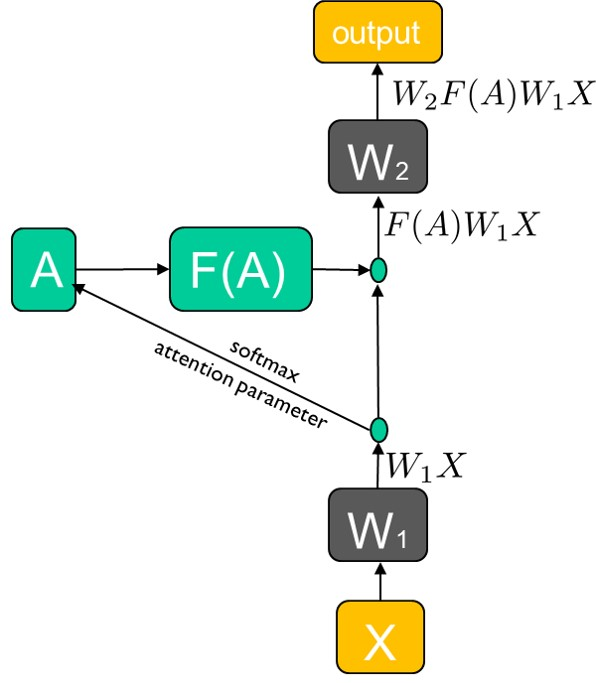
\includegraphics[width=10cm]{theory/4.jpg}
%     \caption{\label{2-4}无向图与邻接矩阵}
% \end{figure}
% \begin{figure}[htbp]
%     \centering
%     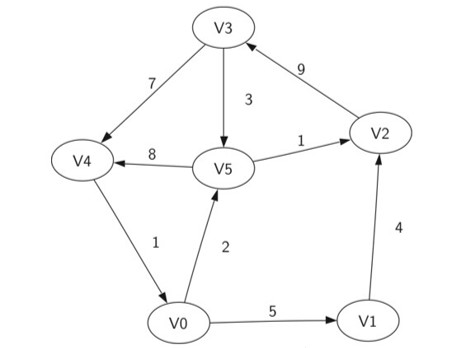
\includegraphics[width=10cm]{theory/5.jpg}
%     \caption{\label{2-5}有向图与邻接矩阵}
% \end{figure}

\begin{figure}[htbp]
    \centering
    \begin{minipage}[t]{0.48\textwidth}
    \centering
    \captionsetup{width=6cm}
    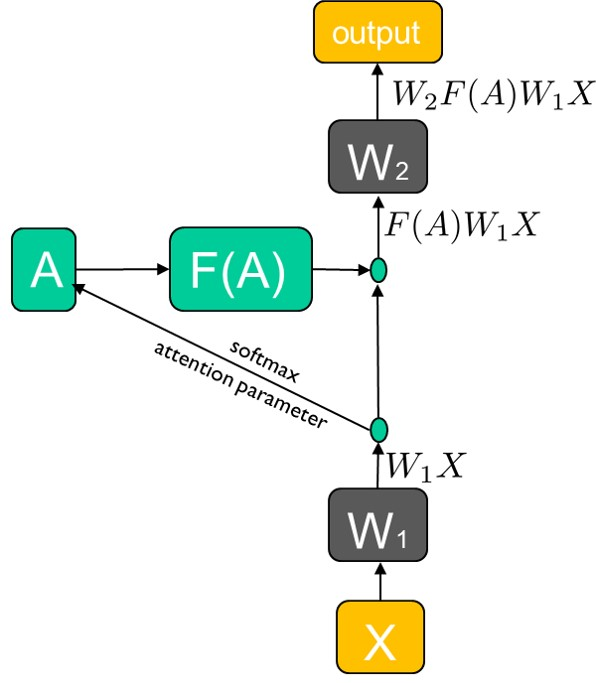
\includegraphics[width=8cm]{theory/4.jpg}
    \caption{\label{2-4}无向图与邻接矩阵}
    \end{minipage}
    \begin{minipage}[t]{0.48\textwidth}
    \centering
    \captionsetup{width=6cm}
    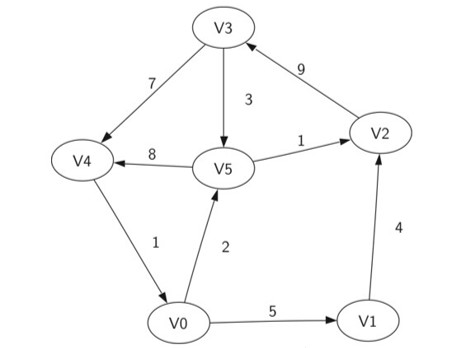
\includegraphics[width=8cm]{theory/5.jpg}
    \caption{\label{2-5}有向图与邻接矩阵}
    \end{minipage}
\end{figure}

\subsection{图信号及其变换}
不失一般性,我们将图信号定义为从节点集合$V$到向量集合$ R^{K} $的映射:
$$ s : V\to R^{K}, \ v_{n} \mapsto s_{n} $$
为了简化表示,我们可以将图信号表示为向量表示$ s = (s_0 \ s_1 \ \cdots  \ s_{N-1})^{T}$,其中的
每个元素$ s_{n} $对应于已知图结构$\ G = (V , E) $中的$ v_{n} $节点。

\begin{figure}[ht]
    \centering
    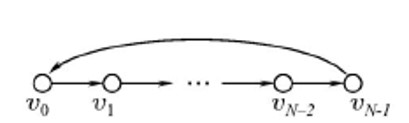
\includegraphics[width=6cm]{theory/9.jpg}
    \caption{\label{2-9}时间序列}
\end{figure}
我们可以将由图信号得到一个新的图信号的过程,定义为图信号变换,或称为图滤波。
图信号变换既可以发生在频域上和时域上,也可以在其他域上。例如,有一个有向循环
图,图上每个节点上的信号,在下一个时刻沿着箭头传到下一个节点,如图\ref{2-9}
所示,其时域上的图信号变换就可以表示为$ \tilde{s} = Cs  $。
\begin{equation*}
    C_{m,n} = \begin{cases}1,if \ n - m = 1 \ mod \ N
    \\0,otherwise
    \end{cases}
\end{equation*}
图信号通过图卷积层的过程,本质上就是图信号变换的过程,设计图卷积层等价于
设计图滤波器,因此,我们能够将图信号处理的理论应用到图卷积神经网络的设计中来。

\subsection{基于频谱理论的图卷积神经网络}
\subsubsection{基本理论}
基于频谱的方法,在图信号处理领域中具有坚实的数学基础。用频谱理论来设计图卷积神经网络,一般适用于无向图。
由已知的邻接矩阵,我们可以得到归一化的图拉普拉斯矩阵,$ L=I_N-D^{-1/2}AD^{-1/2} $,其中A是邻接
矩阵,D是节点的度矩阵 $ D_{ii}={\sum_{j}} A_{ij} $。因为归一化图拉普拉斯矩阵具有
实对称正半定的性质,所以可以将它分解为$ L=U\Lambda U^T $,其中$ U=[u_0,\ldots,u_{n-1}] \in R^{N \times N} $
是特征向量的矩阵,$ \Lambda $是特征值的对角矩阵,$\Lambda_{ii}=\lambda_{i} $。归一化拉普拉斯矩阵的
特征向量构成一个标准正交空间,可用$ UU^{T}=I $表示。

在图信号处理中,图信号$ x\in R^{N} $ 代表图上所有节点的信号, $ x_i $代表第$ i $个节点
上的信号值。对于信号$ x $,我们可以将它的图傅里叶变换可以表示为$ F(x)=U^{T}x $,逆变换可以表示为,
$ F^{-1} (\widehat{x}) = U\widehat{x} $。图傅里叶变换将输入的图信号投影到标准正交空间,在标准正交空间中,
正交基由归一化图的拉普拉斯特征向量构成。从一个角度理解,变换后的信号$ \widehat{x} $的元素是图信号在新空间中的坐标,
所以输入的图信号其实就是$ \widehat{x} $的逆图傅里叶变换,可以表示为$ x = {\sum_{i}}\widehat{x}_{i}u_{i} $。
借助图傅里叶变换的定义,我们可以将输入信号$ x $与滤波器$ g \in R^{N} $的图卷积操作被定义为:
$$ x\ast_{G}g = F^{-1}(F(x) \odot F(g)) = U((U^{T}x) \odot (U^{T}g)) $$
其中$ \odot $为元素的阿达玛乘积。所有基于频谱理论的图卷积神经网络都基于上述的定义。因为$U^{T}$已知,
我们可以等价地认为图滤波器是$ g_{\theta}=diag(U^{T}g) $,那么图卷积操作可以简化表示为:
$$ x\ast_{G}g = U g_{\theta} U^{T} x $$
基于频谱理论的图卷积网络设计,重点就是如何设计图滤波器$ g_{\theta} $。

\subsubsection{三种主要设计方法}
初期在设计图滤波器时[19],我们直接将图滤波器设计为,其中$ g_{\theta} = diag(\theta),\theta \in R^N $, $ \theta $为待学习的参数。
则此时的卷积操作可以表示为,$ y = V g_{\theta} V^{T} x $。这种图滤波器设计方法,缺点是明显的,
当图上节点数量很多(即n的值很大)时,此时将要学习的参数量是很大的,这势必会严重影响图神经网络的效率和表达能力。

后来[20],为了解决图神经网络的参数过多的问题,又出现了利用特征值矩阵$ \Lambda $的矩阵多项式来设计图滤波器的方法。这种方法
将图滤波器表示为,$ g_{\alpha} = {\sum_{i=0}^{K}} \alpha_{i} \Lambda^{i},  \alpha \in R^K $,其中$ \alpha $为需要学习的参数。
则此时的卷积操作可以表示为,$ y = V ({\sum_{i=0}^{K}} \alpha_{i} \Lambda^{i}) V^{T} x $。这种
图滤波器设计方法,明显减少了需学习的参数,但由于计算过程中涉及拉普拉斯矩阵的特征分解,此过程的计算复杂度为$ O(n^{3}) $,
这依然是非常大的运算开销。

同时[20],为了提高训练效率,又提出了用特征值矩阵$ \Lambda $的Chebyshev多项式来设计图滤波器的方法。这种方法将图滤波器表示
为,$ g_{\beta} = {\sum_{i=0}^{K}} \beta_{i} T_{i}(\Lambda),  \beta \in R^K $,其中$ \beta $为需要学习的参数。
则此时的卷积操作可以表示为,$ y = V ({\sum_{i=0}^{K}} \beta_{i} T_{i}(\Lambda)) V^{T} x $。这种图滤波器设计方法,
不需要学习过多的参数,还避免了拉普拉斯矩阵的特征分解,将计算复杂度降到了$ O(n) $。

\subsubsection{频谱理论的特点}
参考上面部分我们所提到的,基于频谱理论的图卷积神经网络的基本理论和设计方法,我们总结了
基于频谱理论的图神经网络的主要特点。
\begin{itemize}
    \item \textbf{无向图} \quad
    因为涉及拉普拉斯矩阵的特征分解,所以频谱理论中适用的图结构必须是无向图。但实际中,还有
    很多有向图的情况,比如交通网络图中,有一些路线可能是只能够单行的。因此,只能处理无向图
    这一特点,很大程度限制了频谱模型在图卷积神经网络的中应用。
    
    \item \textbf{边权重} \quad
    对于频谱理论的设计方法,我们无法学习每条边的权重,邻接矩阵$A$中每条边的权重必须事先确定。
    但是实际中,很多图结构并不是每条连边的权重都是相同的,比如在社交网络中,用户之间的不同关系,
    将直接体现在边权重的不同上。所以,每条边的权重必须事先确定这一特点,限制了基于频谱理论的图神
    经网络的表达能力。

    \item \textbf{泛化能力} \quad
    在基于频谱理论的设计方法中,本质上是用矩阵多项式来拟合图滤波器,那么图结构对拟合的多项式参数
    必然有很直接的影响。然而在现实中,很多图结构并不是固定不变的,比如节点数量的增减和边的连通与否,
    都可能随着时间变化。由于基于频谱理论的图神经网络并没有很强的泛化能力,它不能应用于复杂的场景。

    \item \textbf{运算速度} \quad
    基于频谱理论的图神经网络在训练和测试的过程中,主要的运算开销是高阶多项式矩阵需要进行矩阵之间的
    乘法。而在运算过程中,相乘的矩阵大多是稀疏的,并且Chebyshev多项式用矩阵的加减代替了矩阵的乘法。
    基于频谱理论的图神经网络的训练速度是较快的。
\end{itemize}

\subsection{基于空间理论的图卷积神经网络}
\subsubsection{基本理论}
与传统CNN在图像上的卷积运算类似,基于空间的方法根据节点的空间关系定义图的卷积。图像可以看作是一种
特殊的图结构,每个像素代表一个节点。如图\ref{2-6}a所示,每个像素直接与其附近的像素相连。类似地,基于空
间的图卷积将中心节点的表示与它的邻居的表示进行卷积,以得到中心节点的更新表示,如图\ref{2-6}b所示。从另一
个角度来看,基于空间的图卷积神经网络与递归图神经网络具有相同的信息传递思想。空间图卷积运算本质上是
沿着边传播节点信息。

\begin{figure}[ht]
    \centering
    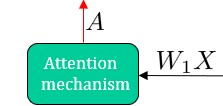
\includegraphics[width=12cm]{theory/6.jpg}
    \caption{\label{2-6}图像上的卷积 vs 图上的卷积}
\end{figure}

注意力机制图神经网络(GAT)[21]是一种最常见的基于空间理论的设计方法,它假设相邻节点对中心节点的贡献既不完全相同
,也不预先确定,这点与频谱理论非常不同(见图\ref{2-7}和图\ref{2-8})。GAT采用注意机制来学习两个连接节点之间的相对权重。
类似于CNN的卷积定义,GAT的图卷积运算定义为:
$$  y = A W x $$
其中,图信号$ x\in R^{F \times N} $代表图上所有节点的信号,$ W \in R^{F' \times F} $是权重矩阵,$A \in R^{N \times N}$是注意力
矩阵,注意力权重$A_{ij}$衡量节点$i$和它相邻节点$j$的连接权重:
$$
    A_{ij} = \frac{exp(L(\vec{a}^{T}[W\vec{x_{i}}||W\vec{x_{j}}]))}
    { {\textstyle \sum_{k\in N_{i} }^{}} exp(L(\vec{a}^{T}[W\vec{x_{i}}||W\vec{x_{k}}]))}  
$$
其中,$\vec{a} \in R^{2F'}$是一个需要学习的注意力参数,$ || $是一个将两个向量拼接的运算,$ N_{i} $表示节点$i$的
相邻的节点集,$L$表示LeakyReLU函数,softmax函数保证了节点$i$所有邻居的注意权值总和为$1$。

\begin{figure}[htbp]
    \centering
    \begin{minipage}[t]{0.48\textwidth}
    \centering
    \captionsetup{width=5cm}
    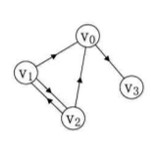
\includegraphics[width=6cm]{theory/7.jpg}
    \caption{\label{2-7}基于频谱理论的图卷积神经网络,在卷积的过程中预先显式地确定边权重$A_{ij}$。}
    \end{minipage}
    \begin{minipage}[t]{0.48\textwidth}
    \centering
    \captionsetup{width=5cm}
    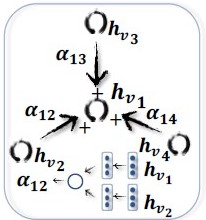
\includegraphics[width=6cm]{theory/8.jpg}
    \caption{\label{2-8}基于空间理论的图卷积神经网络,隐式地捕捉边权重$A_{ij}$,所以越重要的节点能获得越大的权重。}
    \end{minipage}
\end{figure}

\subsubsection{空间理论的特点}
与基于频谱的图卷积神经网络相比,基于空间理论的图卷积神经设计方法有其独有的优缺点,现将其总结如下。
\begin{itemize}
    \item \textbf{有向图} \quad
    因为基于空间理论的设计方法,不需要注意力权重$A_{ij}$和$A_{ji}$严格地相同,所以GAT可以
    支持有向图的图结构。所以在搭建图卷积神经网络的过程中,GAT在图结构的表示上有更加强大的表达
    能力,可以适用更加丰富的场景。
    
    \item \textbf{边权重} \quad
    基于空间理论的图卷积神经网络的边权重,表示为$ A $注意力权重矩阵中的元素$A_{ij}$。
    $A_{ij}$是不需要事先确定的,而是借助学习$ \vec{a} $的注意力参数得到的。所以,通过自主
    学习边权重,GAT在图结构的边权重表示上有更加强大的表达能力。

    \item \textbf{图结构的hop} \quad
    空间理论的设计中,注意力矩阵$ A $中的元素$A_{ij}$仅在具有相邻关系的节点之间有值,
    这使得GAT的图结构的$ hop=1 $。然而在频谱理论中,我们能够通过多项式阶数$ K $的选择来自主
    确定图结构的$ hop $,所以与频谱理论相比,空间理论对图结构里间接相连节点间的关系的表达能力偏弱。

    \item \textbf{运算速度} \quad
    对于基于空间理论的设计方法而言,需要训练的参数是$ \vec{a} \in R^{2F'} $,$F'$的值一般较小,
    所以需要训练的参数数量并不是很多。但是因为$ \vec{a} $在每个边权的学习中都会使用,所以依旧
    需要很长的训练时间,GAT相较于基于频谱理论的神经网络效率偏低。

\end{itemize}